\section{\glsentrylong{ss}}
\label{sec:ssharp}

\gls{ss} ist ein am \isse der Universität Augsburg entwickeltes Framework zum modellbasierten Testen und Verifizieren von Systemen.
Entwickelt wurde das Framework mithilfe des .NET"=Frameworks und der Sprache \cS, die auch zum Entwickeln der zu testenden Modelle genutzt werden.
Dadurch können zahlreiche Funktionen des .NET"=Frameworks bzw. der Sprache \cS im Speziellen genutzt werden.
\gls{ss} vereint dabei die Simulation, die Visualisierung, modellbasierte Tests sowie die Verifizierung der Modelle durch einen \gls{MCr} \cite{Habermaier2015,Habermaier2016}.
Dadurch können alle Schritte einer vollständigen Analyse inkl. Modellierung auch direkt im Visual Studio ausgeführt werden und somit auch die Funktionen der IDE und .NET, wie \zB die Test- und Debugging"=Werkzeuge, genutzt werden.
Um korrekte Analysen zu gewährleisten, hat \gls{ss} jedoch auch einige Einschränkungen, wodurch \zB Schleifen und Rekursionen nur eingeschränkt bzw. nicht möglich sind.
Eine der größten Einschränkungen ist allerdings, dass während der Laufzeit eines Tests durch \gls{ss} keine neuen Objektinstanzen innerhalb des zu testenden Modells erzeugt werden können, sodass alle benötigten Instanzen bereits während der Initialisierung des Modells erzeugt werden müssen \cite{Habermaier2015}.

\subsection{Aufbau eines Modells}
\label{subsec:ssharpModel}

Um ein System testen zu können, muss dieses zunächst modelliert werden.
Die dafür verwendeten Modelle sind meist stark vereinfacht und bilden nur die wesentlichen Aspekte der realen Systeme ab.
Für einen korrekten Test ist es jedoch wichtig, dass das Modell des Systems vergleichbar mit dem echten System ist.
Da \gls{ss} mithilfe von .NET und der Sprache \cS entwickelt wurde, können entsprechend zahlreiche Funktionen hiervon zum Entwickeln des Modells genutzt werden.
Die Modelle sind dadurch einerseits ganz normale, ausführbare C\#"=Programme, stellen andererseits aber auch Modelle von realen, oftmals sicherheitskritischen, Systemen dar \cite{Habermaier2016}.

Folgendes Beispiel zeigt den typischen, grundlegenden Aufbau einer \gls{ss}-Komponente:

\begin{lstlisting}[label=lst:ssExample,style=cs,
caption={Grundlegender Aufbau einer \glsentryshort{ss}"=Komponente.}]
public class YarnNode : Component
{
  // fault definition, also possible: n§§ew PermanentFault()
  public readonly Fault NodeDeadFault = new TransientFault();
  
  // interaction logic (Fields, Properties, Methods...)
  
  // fault effect
  [FaultEffect(Fault = nameof(NodeDeadFault))]
  internal class NodeDeadFaultEffect : YarnNode
  {
    // fault effect logic
  }
}
\end{lstlisting}

Jede Komponente des Modells muss von \texttt{Component} erben, um als \gls{ss}"=Komponente definiert zu sein.
Sie kann dabei einen oder mehrere Komponentenfehler enthalten, die bei dieser Komponente auftreten können, im Beispiel in \cref{lst:ssExample} ist dies \texttt{NodeDeadFault}, der den Ausfall eines Nodes herbeiführt.
Ein Komponentenfehler kann dabei temporär (\texttt{TransientFault}) oder dauerhaft (\texttt{PermanentFault}) sein.
Der Effekt eines Komponentenfehlers wird in der entsprechenden Effekt"=Klasse definiert, welche von der Hauptklasse (hier \texttt{YarnNode}) erbt und mithilfe des Attributs \texttt{FaultEffectAttribute} dem dazugehörigen Komponentenfehler zugeordnet wird \cite{Habermaier2016,Habermaier2015}.
Neben den eigentlichen Komponenten enthält jedes Modell zudem eine zentrale \texttt{Model}"=Klasse, die von \texttt{ModelBase} erbt.
Sie stellt die zentrale Schnittstelle zwischen \gls{ss} und dem Modell selbst dar und wird zur Ausführung bzw. der Analyse des Systemmodells durch \gls{ss} benötigt \cite{SSWikiModels}.

Das Systemmodell kann nach der Modellierung vom \gls{ss}"=Compiler kompiliert werden und bindet sich mithilfe der \gls{ss}"=Laufzeitumgebung nach folgendem Schema in die grundlegende Architektur des Testens mit \gls{ss} ein:

\begin{figure}[h]
    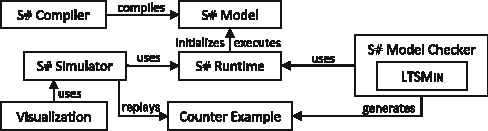
\includegraphics{./resources/ssharpArchitecture.pdf}
    \caption[Grundlegende Architektur eines Tests mit \glsentryshort{ss}]
    {Grundlegende Architektur eines Tests mit \gls{ss} (entnommen aus \cite{Habermaier2016})}
    \label{fig:ssharpTestApproach}
\end{figure}

Zur Ausführung eines \gls{ss}"=Modells gibt es neben der Simulation und dem \gls{MCr} zusätzlich noch die Möglichkeit der Ausführung mithilfe der \gls{DCCA} (vgl. \cref{subsec:ssharpExecution}).
Alle drei Ausführungswerkzeuge führen auf jeweils ihre Art das entwickelte Modell aus.
Dabei werden die Gegenbeispiele dazu genutzt, um mit deren Hilfe die benötigte Fehlermenge im Modell zu ermitteln, bei der das gesamte System ausfällt \cite{Habermaier2016}.

Ein \gls{ss}"=Modell enthält jedoch auch noch weitere Bestandteile, was sich vor allem beim Ansatz des Back"=to"=Back"=Testings mithilfe der \gls{DCCA} zeigt:

\begin{figure}[h]
    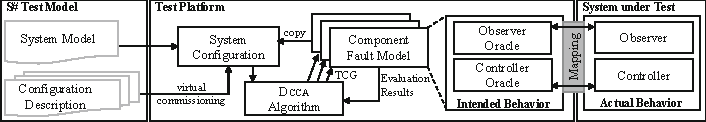
\includegraphics[width=\columnwidth]{./resources/b2bTestApproach.pdf}
    \caption[Ansatz des Back"=to"=Back"=Testings mit \glsentryshort{ss}]
    {Ansatz des Back"=to"=Back"=Testings mit \gls{ss} (entnommen aus \cite{Eberhardinger2016})}
    \label{fig:ssharpB2BTesting}
\end{figure}

Um solche Tests durchzuführen, benötigt das Modell weitere Komponenten.
Der \emph{Controller} dient vor allem dazu, um das System zu steuern, während der \emph{Observer} das System überwacht und dem Controller die benötigten Daten bereitstellt.
Mithilfe eines \emph{Oracle}s wird geprüft, ob sich das System im Verlauf des Tests so verhält, wie es erwartet wird.
Hierfür werden im Modell \emph{Constraints} definiert, welche die Implementierung der Anforderungen an das \gls{SuT} im Modell darstellen und bei der Ausführung durch das Oracle validiert werden.
Dadurch kann automatisiert ermittelt werden, ob sich das \gls{SuT} wie erwartet verhält \cite{Eberhardinger2016,Habermaier2015}.

Für weitere Informationen zum Aufbau eines \gls{ss}"=Modells sei an dieser Stelle auf entsprechende Literatur \cite{Eberhardinger2016,Habermaier2015,Habermaier2016}, sowie auf die Dokumentation von \gls{ss} \cite{SSWiki} verwiesen.

\subsection{Ausführung eines Modells mit \glsentryshort{ss}}
\label{subsec:ssharpExecution}

Um die Modelle zu testen, kommen in \gls{ss} verschiedene Werkzeuge zum Einsatz.
Eines davon ist eine reine Simulation, bei der das Framework nur einen Ausführungspfad ausführt und dabei keine Komponentenfehler aktiviert bzw. die Aktivierung \emph{manuell} durch \emph{eigenen} Code im entwickelten Modell gesteuert werden kann.
Ein weiterer Nutzen liegt in der Möglichkeit, im ausgeführten Ausführungspfad zeitliche Abläufe zu berücksichtigen, da hier das Modell schrittweise ausgeführt wird.
Hierbei wird für jede im Modell genutzte Komponente pro Schritt einmal die jeweilige Methode \texttt{Update()} aufgerufen, in der die jeweiligen Komponenten ihre Aktivitäten durchführen \cite{Habermaier2016}.

Das zweite Werkzeug zur Ausführung von Modellen in \gls{ss} ist der \gls{MCr}.
Hierbei kann der in \gls{ss} enthaltene, oder alternativ \emph{LTSmin}\footnote{\url{http://ltsmin.utwente.nl/}} genutzt werden \cite{SSWikiModelChecking,Habermaier2016}.
Beim \gls{MC} werden in einem \emph{brute-force}-ähnlichem Verfahren alle möglichen Zustände und Ausführungspfade in einem Modell mit einer endlichen Anzahl an Zuständen getestet.
Dadurch wird es ermöglicht, verschiedene Eigenschaften eines System zu testen und Fehler (\zB Deadlocks) zu erkennen \cite{Grumberg1999}.

Ein weiteres, wichtiges Werkzeug von \gls{ss} ist die \gls{DCCA}, welche eine vollautomatische und \gls{MC}-basierte Sicherheitsanalyse ermöglicht (Back"=To"=Back"=Testing).
Dabei wird durch die \gls{DCCA} die Menge der aktivierten Komponentenfehler ermittelt, mit denen das \gls{SuT} nicht mehr rekonfiguriert werden kann und somit ausfällt.
Je nach Konfiguration können dazu auch Heuristiken genutzt werden, welche die Analyse beschleunigen und genauer machen können \cite{Eberhardinger2016}.
Dabei werden die verschiedenen aktivierten Komponentenfehler während der Analyse in tolerierbare und nicht"=tolerierbare Fehler unterschieden.
Tolerierbare Komponentenfehler werden dazu genutzt, die Grenzen der Selbstkonfiguration des Systems zu ermitteln.
Hierbei wird für jeden Systemzustand nach einer Rekonfiguration durch die \gls{DCCA} eine neue Fehlermenge ermittelt, mit der das System gerade noch lauffähig ist.
Das Auftreten eines tolerierbaren Komponentenfehlers ist also gleichbedeutend mit einem einfachen Fehler im System, welcher die gesamte Funktionsweise des Systems nicht massiv einschränkt und eine weitere Rekonfiguration noch ermöglicht.
Sobald jedoch ein Fehler auftritt, durch den eine Rekonfiguration des Systems nicht mehr möglich ist, wurde ein nicht"=tolerierbarer Fehler gefunden, durch den das System nicht mehr funktionsfähig ist \cite{Habermaier2015}.
